\documentclass{article}

\usepackage{wrapfig}
\usepackage{lmodern}
\usepackage[T1]{fontenc}
\usepackage[spanish]{babel}
\usepackage{mathtools}
\usepackage{graphicx}
\usepackage[utf8]{inputenc}
\usepackage{hyperref}
\usepackage{fancyhdr,lipsum}


\hypersetup{
    colorlinks=true, %set true if you want colored links
    linktoc=all,     %set to all if you want both sections and subsections linked
    linkcolor=blue,  %choose some color if you want links to stand out
}



\title{Documentación \\\large \textbf{Gigabyte B550 Aorus Master}}
\author{Antonio Muñoz Cubero}
\date{20 de Ocutbre de 2020} 


\begin{document}
  \maketitle
    \pagenumbering{gobble}

  \begin{figure}[h]
    \centering
    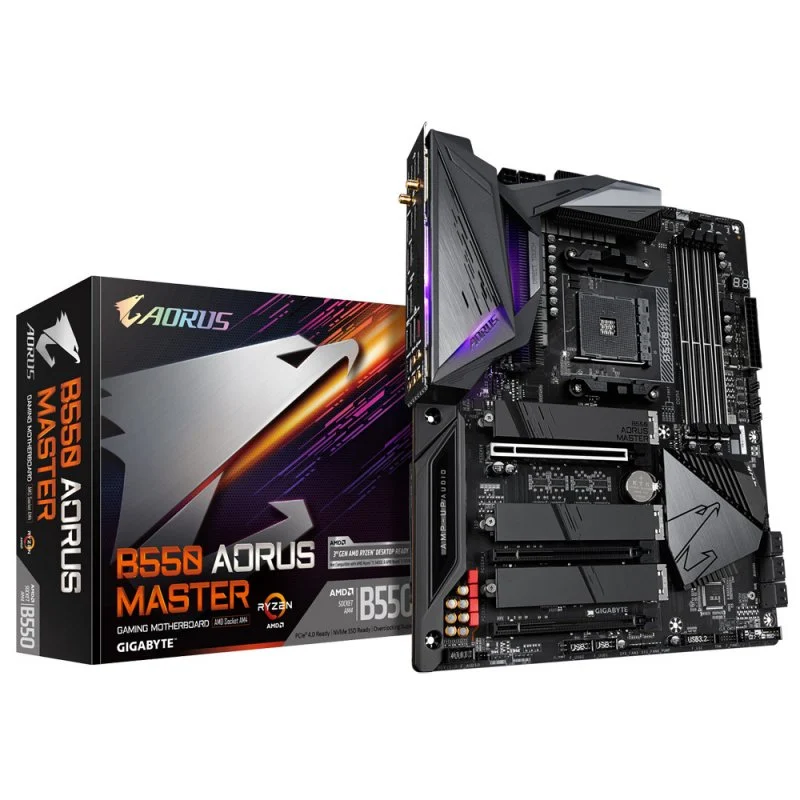
\includegraphics[scale = 0.5]{img/portada.png}
  \end{figure}

\pagestyle{fancy} 
  \newpage
    \tableofcontents
      \lhead[Documentación Placa Base]{Documentación Placa Base}
      \lfoot[IES Francisco De Los Rios]{IES Francisco De Los Rios}
        \pagenumbering{roman}

  \section{Introducción}
    Este documento contiene información sobre la placa base \textbf{B550 AORUS Master} montada por el gigante eléctrónico \textbf{Gigabyte}, esta placa introduce un nuevo chipset, que más adelante entraremos en detalle sobre el, 
    el \text{B550} 
    que permite montar los nuevos procesadores de \textit{AMD}, la serie 3000 y 4000.\\
    Lo bueno de este chipset es que tiene un precio más ajustado al no pertenecer a la serie tope de gama de chipset y nos permite utilizar la tecnología del \textbf{PCIE 4.0}, que mas adelante desarrollaremos y entraremos en 
    detalle, también 
    disponemos de vaías para montar \textbf{discos duros M.2} y otras prestaciones que empezaremos a describir a continuación.

  \newpage
    \section{Características}
      A continuación muestro una tabla con las especificanoes técnicas de la Placa Base, mas adelante iremos centrandonos en cada uno de sus aspectos.
      \begin{figure}[h]
        \centering
        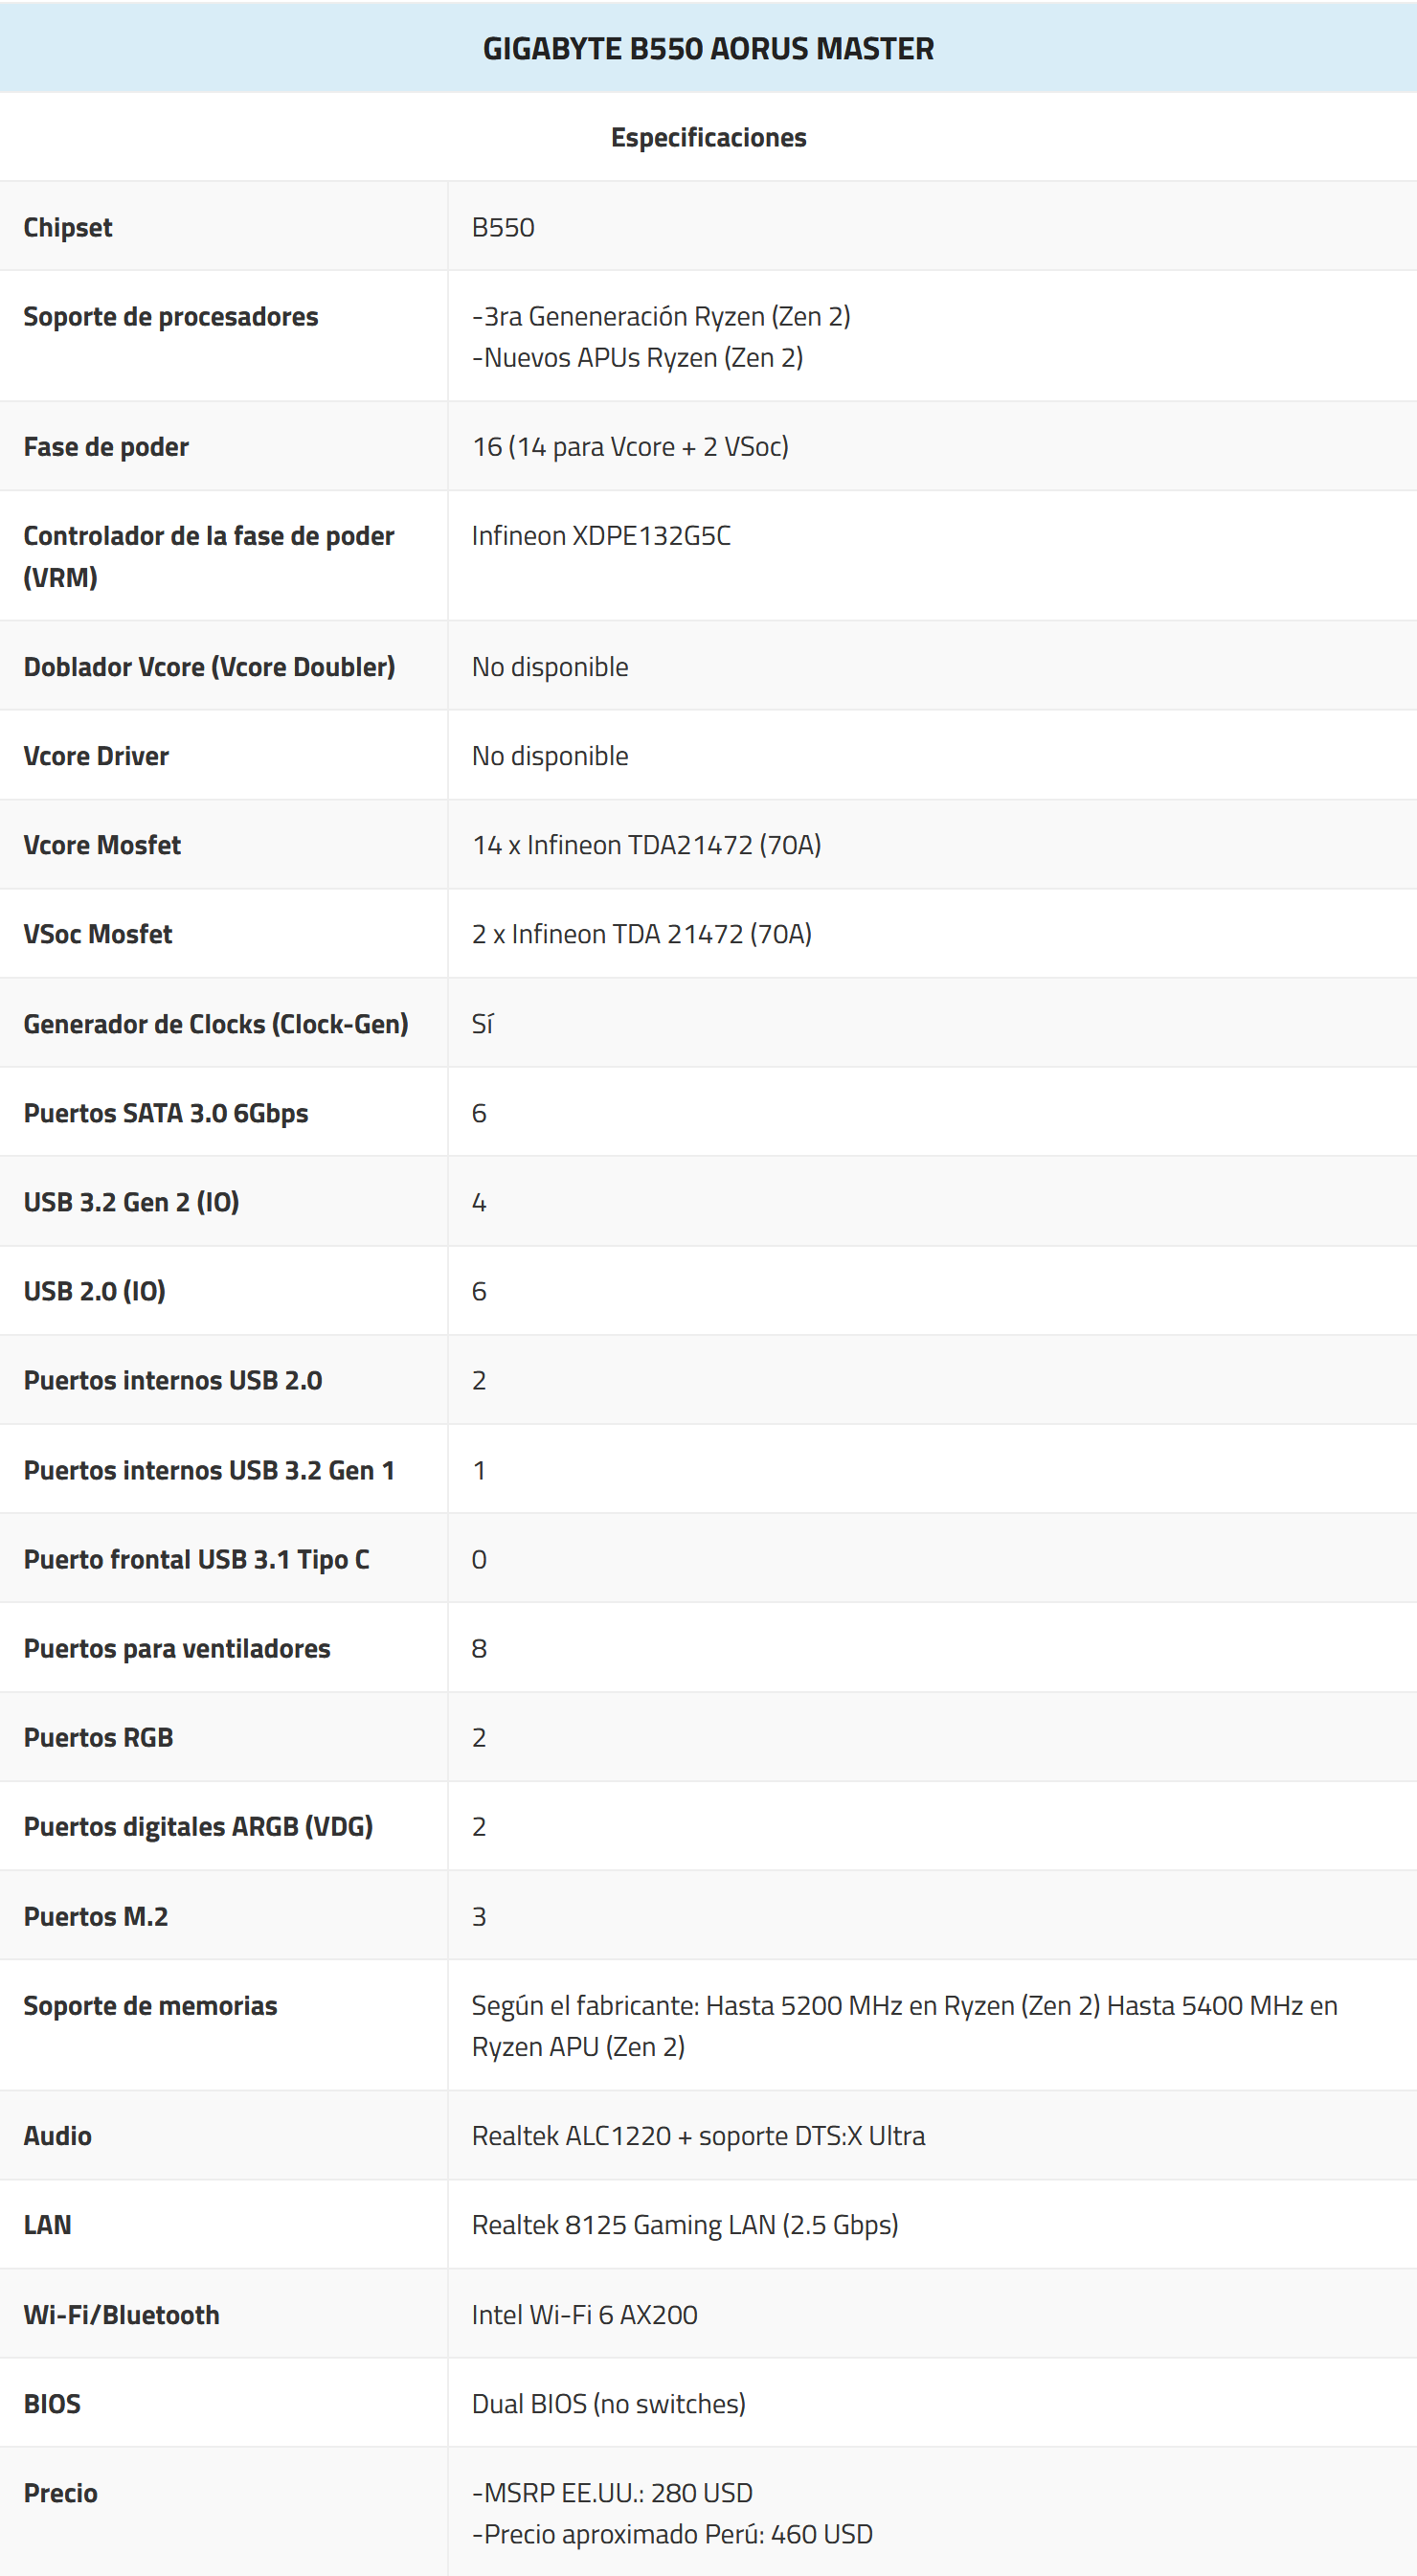
\includegraphics[scale = 0.21]{img/final_specs.png}
      \end{figure}

  \newpage
    \subsection{Memoria RAM}
      Es normal que admita hasta 128 GB de RAM DDR4 a través de sus cuatro módulos DIMM con soporte para Dual Channel. Pero es que gracias al nuevo sistema de conexión daisy chain soportará memorias de hasta 5400 MHz con perfiles XMP. 
      Concretamente será un soporte para esta velocidad en los nuevas APU Ryzen 4000 Zen 2 y de 5200 MHz para los Ryzen 3000 Zen 2.
      \begin{figure}[h]
        \centering
        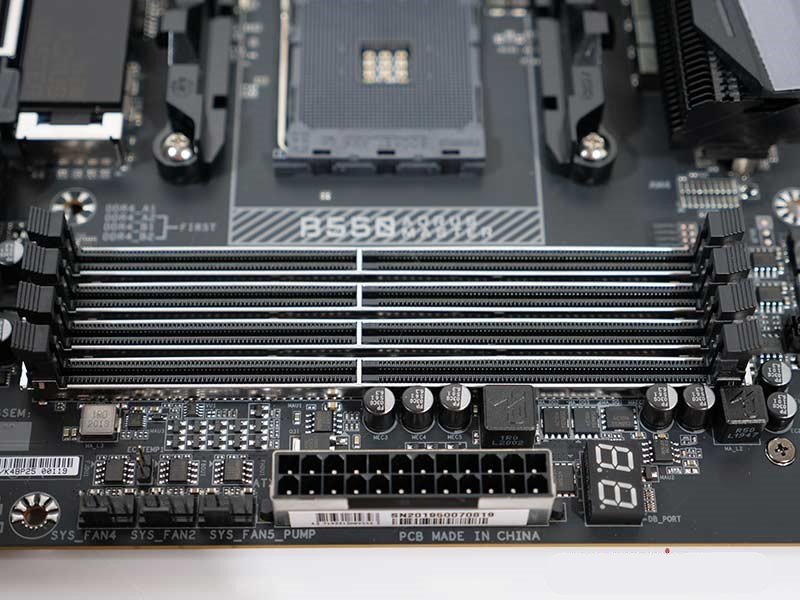
\includegraphics[scale = 0.5]{img/slots.jpg}
        \caption{Slots para memoria RAM}
      \end{figure}     
      \begin{itemize}
        \item Procesadores 3rd Gen AMD Ryzen™: Support for DDR4 5200(O.C.) / 5000(O.C.) / 4866(O.C.) / 4600(O.C.) / 4400(O.C.) / 4000(O.C.) / 3600(O.C.) / 3333(O.C.) /3200/2933/2667/2400/2133 MHz 
        \item Nueva generación AMD Ryzen™ con Procesadores Gráficos Radeon™: Support for DDR4 5400(O.C.) / 5200(O.C.) / 5000(O.C.) / 4866(O.C.) / 4600(O.C.) / 4400(O.C.) / 4000(O.C.) / 3600(O.C.) / 3333(O.C.)
        \item Soporta frecuencias de /3200/2933/2667/2400/2133 MHz 
        \item Arquitectura de memoria Dual channel 
        \item Soporte para ECC Un-buffered DIMM 1Rx8/2Rx8 
        \item Soporte para non-ECC Un-buffered DIMM 1Rx8/2Rx8/1Rx16 
        \item Soporte para Extreme Memory Profile (XMP)
      \end{itemize}
  \newpage
    \subsection{Conexiones Internos}
      \textbf{Listado de conexiones internas:}\\
      \normalsize
          \begin{minipage}{0.5\textwidth}
            \begin{itemize}% never number things manually!
              \item 1 x 24-pin ATX conector de energía principal
              \item 1 x 8-pin ATX 12V conector de energía
              \item 1 x 4-pin ATX 12V conector de energía
              \item 1 x conector para ventilador de la CPU
              \item 1 x conector para refrigeración líquida de la CPU
              \item 4 x conectores para los ventiladores del pc
              \item 2 x conectores para la refrigeración líquida
              \item 2 x conectores para tira led direccionables
              \item 2 x conector para tiras led RGB
              \item 1 x conector para conectores led RGB de la CPU
              \item 3 x conectores de socket M.2
              \item 6 x conectores SATA 6Gb/s
              \item 1 x conectores del panel frontal (energía)
              \item 1 x conectores del panel frontal (audio)
              \item 1 x conectores USB 3.2 Gen 1 
              \item 2 x conectores USB 2.0/1.1 
              \item 1 x sensor detector de ruido
              \item 1 x TPM (Trusted Platform Module)
              \item 1 x Limpiador de la  CMOS
              \item 2 x Sensores de temperatura
            \end{itemize}
          \end{minipage}
          \begin{minipage}{\textwidth}
            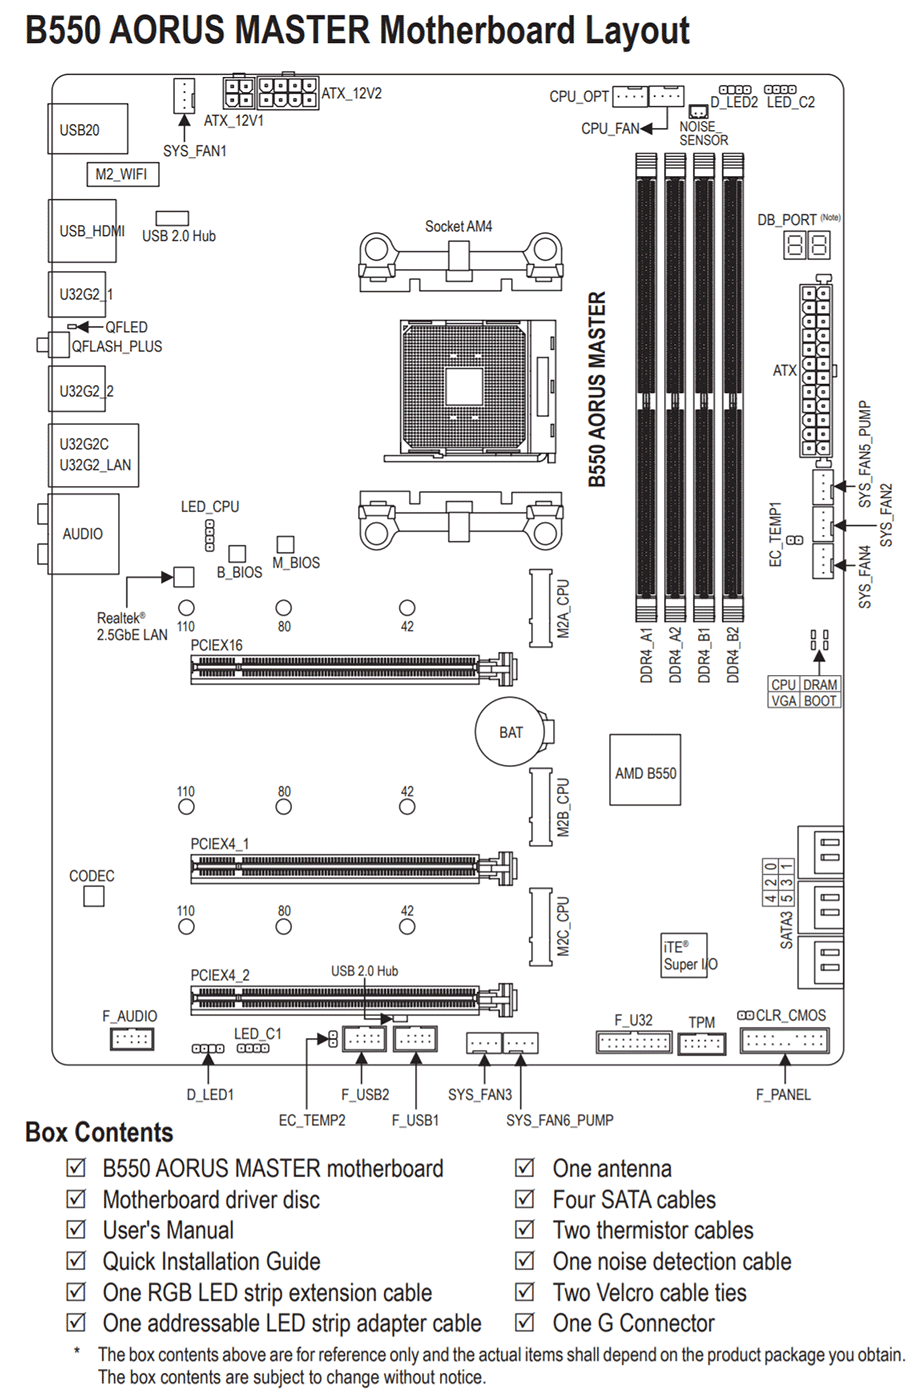
\includegraphics[scale=0.25]{img/B550AORUSMasterDiagram.png}
          \end{minipage}
        

  \newpage
    \subsection{Conectores Externos}
      \normalsize
        {\bfseries Ahora listaré los Conectores Externos de la placa. Estos los usamos para sacar las señales de audio, video, red y demás conexiones.}
        \begin{itemize}
          \item Lista de Conexiones:

          \begin{minipage}{0.5\textwidth}
            \begin{itemize}% never number things manually!
              \item x1 HDMI
              \item x6 USB 2.0/1.1
              \item X5 USB 3.2 GEN2 TYPE A
              \item X1 USB TYPE C
              \item Q-Flash Plus button
              \item X1 puerto RJ-45
              \item X5 AUDIO JACK 
              \item x1 OPTICAL S/PDIF 
            \end{itemize}
          \end{minipage}
          \begin{minipage}{\textwidth}
            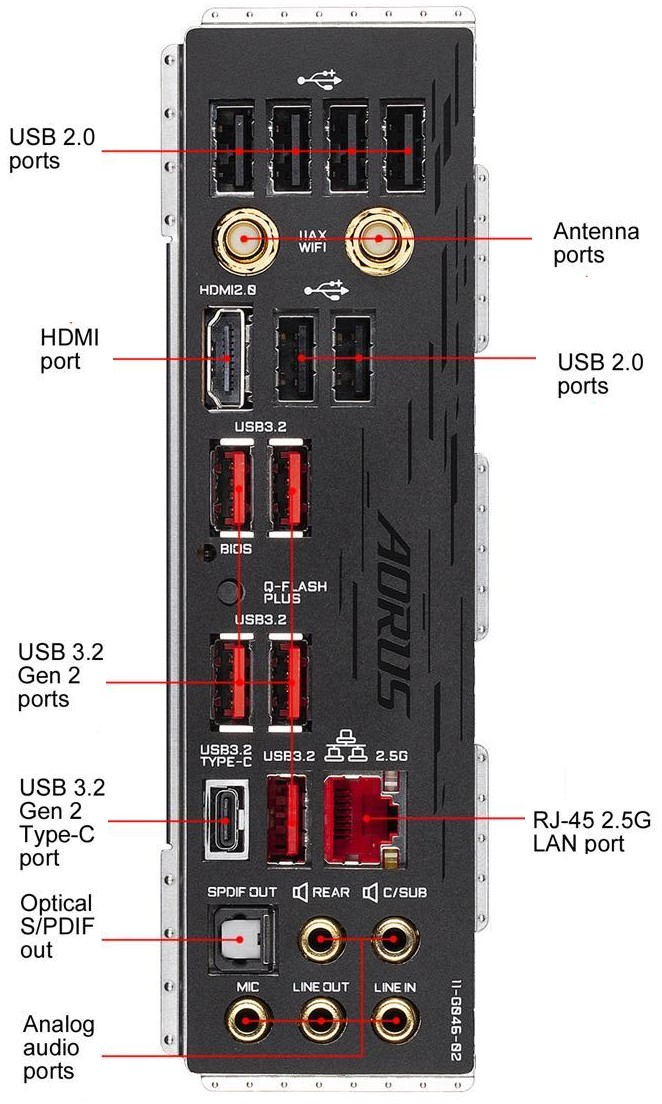
\includegraphics[scale=0.4]{img/frontal_vertical.jpg}
          \end{minipage}
        \end{itemize}
  \newpage

    \subsection{Gráfico de la Placa Base}

        \begin{figure}[h]
          \centering
          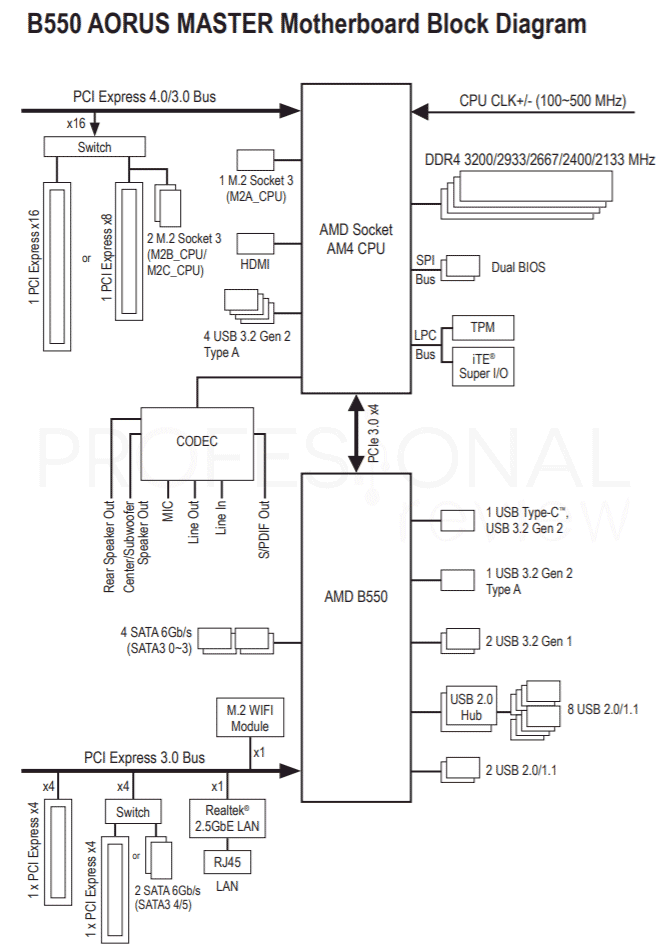
\includegraphics[scale = 0.4]{img/block_diagram.png}
          \caption{Diagrama de bloque de la placa base}
        \end{figure}
        
  \newpage
        \begin{figure}[h]
          \centering
          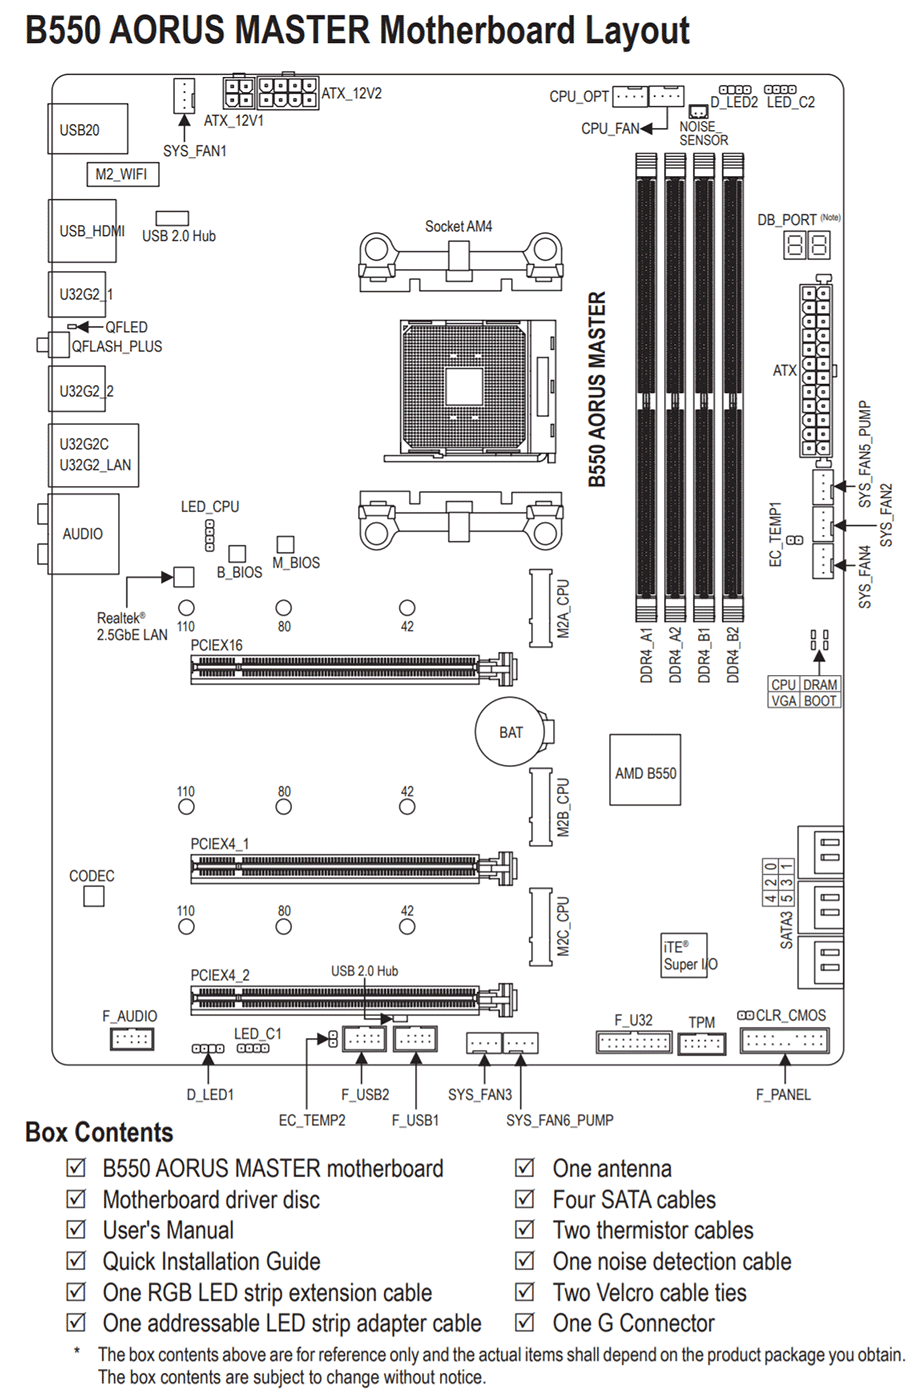
\includegraphics[scale = 0.3]{img/B550AORUSMasterDiagram.png}
        \end{figure}

  \newpage

    \subsection{Procesador}
      La placa base \textit{Aorus B550 Master} tiene capacidad para soportar procesadores de \textbf{Socket AM4} del fabricante \textit{AMD} la serie \textbf{Ryzen 3000 y 5000}  y soporta la nueva gama de procesadores 
      con \textit{Radeon Graphics Processors}.
      El \textbf{chipset} como biene indicando en el nombre de la placa es el \textbf{B550}.
      
    
    \subsection{Periféricos Integrados}
      \subsubsection{Tarjeta Gráfica}
        La Placa Base nos permite hacer uso de los \textbf{gráficos integrados} de las \textit{APU} usando un puerto HDMI que viene integrado en ella, sacando una resolución máxima de \textit{4096 x 2160 a 60 Hz}.
        
      \subsubsection{Tarjeta de Sonido}
        Por otro lado tenemos una \textbf{tarjeta de sonido} integrada en la Placa Base, esta es la \textit{Realtek® ALC1220-VB codec}.  Soporte sonido en alta definición con hasta 8 canales disponibles en 7.1 entregando 
        120 dBA SNR y amplificador de auriculares inteligente para detectar de forma automática su impedancia. La sensibilidad en las entradas de micro delantera y trasera serán de 110 y 114 dBA SNR respectivamente. 
        Finalmente este codec soporte DTS: X Ultra, un encoder que genera sonido 3D en alta calidad especialmente diseñado para juegos.
        
      \subsubsection{Tarjeta de Red}
        Por último, y algo de lo más destacable en esta placa, es que viene provista de una \textbf{tarjeta de red con doble interfaz}, esto nos permite hacer uso de una conexión tanto \textbf{ethernet} como \textbf{wifi} 
        sin necesidad de adaptadores o tarjetas de red extra.
        \\ 
        En el caso de la conectividad \textit{LAN Ethernet}, dispone de un puerto \textbf{RJ45} conectado a un chip \textbf{Realtek RTL8125} que entrega hasta \textbf{2,5 Gbps}. 
        Estas son buenas noticias de cara a las redes internas de alto rendimiento, pudiendo aprovechar este gran ancho de banda para NAS, o en switch o router de gama alta para partidas en red.
        \\
        Junto al enlace cableado tenemos una interfaz inalámbrica Wi-Fi 6 a través de una \textbf{tarjeta 2230 M.2 CNVi Intel AX200}. Las prestaciones de red son las ya conocidas por muchos, con una conexión Dual Band 2×2 con MU-MIMO 
        y OFDMA que \textbf{eleva el ancho de banda en 5 GHz hasta los 2404 Mb/s y en 2,4 GHz hasta 574 Mb/s}. A esta se le suma la interfaz Bluetooth 5.0, aunque debemos saber que la versión más actual de tarjeta es la \textbf{AX201} 
        que añade BT 5.1, aunque solo se usa en placas Intel Z490. Para exprimir este ancho de banda necesitaremos un router Wi-Fi 6 por supuesto.
  \newpage
    \subsection{Fases de Alimentación}
      La primera etapa de suministro de energía consiste en dos conectores de \textbf{tipo EPS}, uno de ellos con 4 pines y el otro completo con 8. Estas cabeceras están reforzadas con acero y cuentan con pines de metal sólido para mejorar la 
      entrega de corriente.
      \\
      \begin{figure}[h]
        \centering
        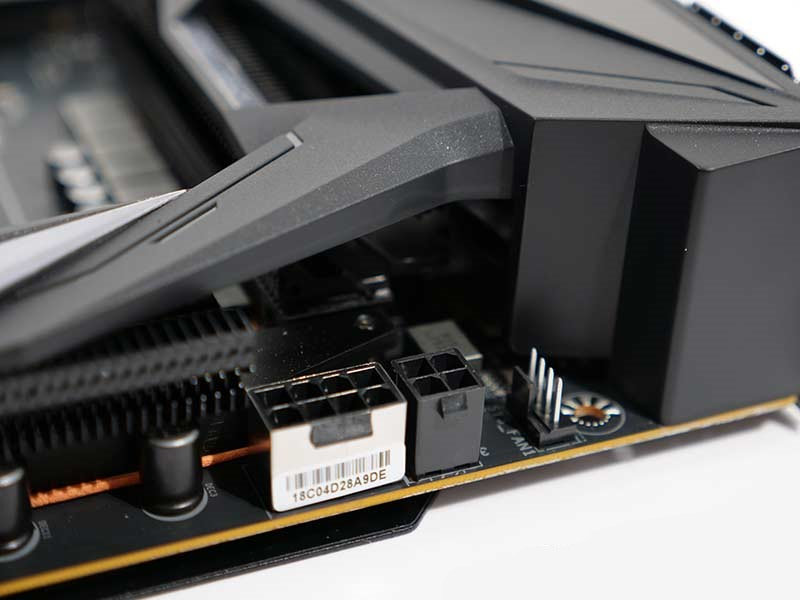
\includegraphics[scale=0.35]{img/alimentación1.jpg}
        \caption{Pines de alimentación de la placa}
      \end{figure}
      \\
      La segunda fases de potencia y conversión AC – DC se salda con esos \textbf{16 MOSFETS Infineon TDA21472 de 70} de gran calidad. Estas etapas de potencia de 3 estados 
      cuentan con telemetría integrada de corriente y temperatura, \textit{suministrando un voltaje de salida de entre 0,25 y 5,5V, teniendo una alta frecuencia de conmutación de 1,5 MHz}.
     
      \begin{figure}[h]
        \centering
        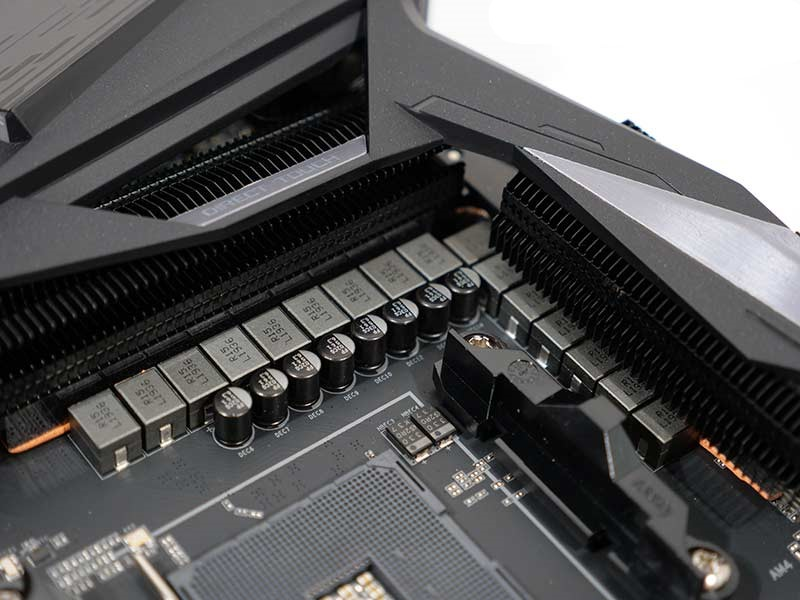
\includegraphics[scale=0.35]{img/alimentación2.jpg}
        \caption{MOSFETS de la placa base}
      \end{figure}

      Los \textbf{MOSFETS} estarán gestionados por una EPU o controlador digital \textbf{Infineon XDPE132G5C PWM}. Este elemento proporciona el ajuste individual de cada convertidor con una señal digital directa, ya que en este caso no tenemos 
      duplicadores de señal y tampoco señales paralelas, y por tanto las fases serán reales. Para el alisado de la señal eléctrica se utilizando 16 Chokes metálicos y condensadores sólidos. 

  
      \section{Consejos de Instalación}
        La Placa Base y la gran mayoría de componentes electrónicos de nuestro PC son muy sensibles a la \textit{electricidad estática}, teniendo esto en cuenta, si no nos andamos con cuidado, una errónea manipulación del material
        puede llevar a que estropeemos el mismo. Por ello, una gran recomendación es usar una \textbf{pulsera antiestática} para prevenir a nuestro equipo de dichos peligros.
        \\
        Otro consejo que puedo dar como experiencia personal, es instalar el \textbf{CPU} antes de meter la placa en la torre y atornillarla, es bastante más cómodo, así como la \textbf{RAM}. Tener localizados los conectores de 24 y 16 pines para 
        instalar más rapido la placa y sus componentes.

        \begin{figure}[h]
            \centering
            
\includegraphics[scale = 0.5]{img/pulsera.jpg}
            \caption{Pulsera antiestática}
        \end{figure}
    
     \newpage   
      \section{BIOS}
        \subsection{Configuración de la BIOS}
          Primero de todo, mostraremos como acceder a la BIOS de nuestr Placa Base. En primer lugar, accedemos la \textbf{BIOS} pulsando la tecla \textit{'DEL'} y una vez dentro cabe destacar que hay dos modos de la \textit{BIOS}, que podemos alternar 
          pulsando \textit{'F2'}.
          \begin{figure}[h]
            \centering
            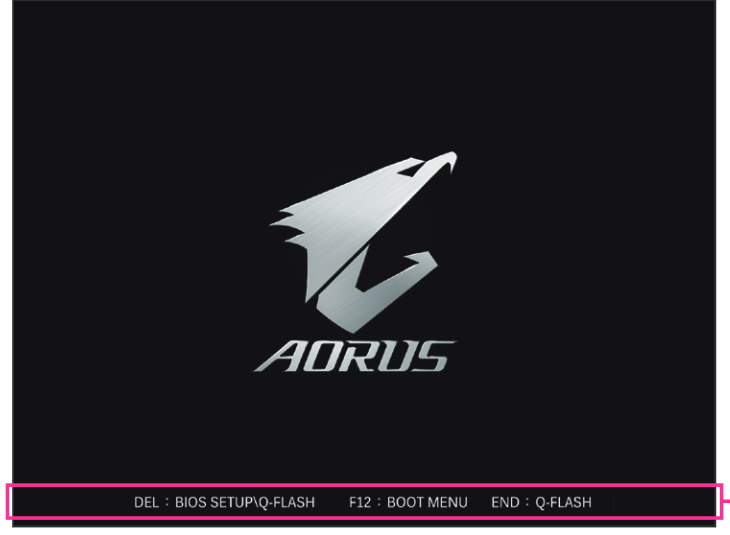
\includegraphics[scale = 0.5]{img/BIOS_START.png}
            \caption{Pantalla de Inicio de la Placa Base}
          \end{figure} 
          En la versio \textbf{EASY}, pudes usar el cursor del ratón para ir navegando por los diferentes apartados, sin embargo, esta es más limitada, pero en la version \textbf{ADVANCED} podemos nos provee los detalles de la configuración de la \textit{BIOS}.
          \\\\
          AORUS ha renovado notablemente la interfaz de su BIOS, que en este caso dispone de una configuración doble BIOS con un CMOS de respaldo para otra configuración o fallos en overclocking. Como es habitual en otras UEFI, tenemos un modo fácil y 
          avanzado, para así poder acceder a los parámetros más genéricos en usuarios que no desean hacer overclocking, y los más avanzados en caso contrario.\\
        \newpage          
          \begin{figure}[h]
            \centering
            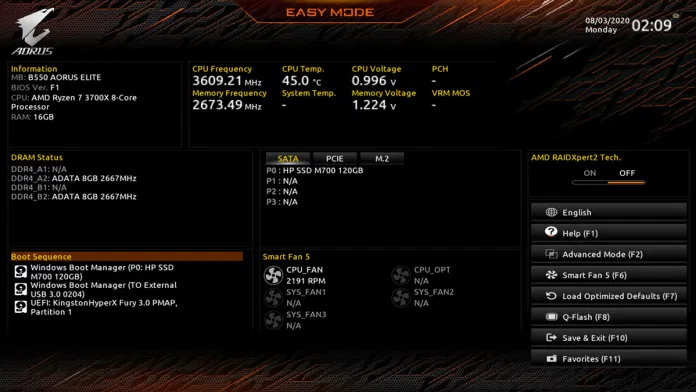
\includegraphics[scale = 0.5]{img/BIOS1.png}
            \caption{Interfaz gráfica de la BIOS}
          \end{figure}
          De un vistazo podremos ver bastantes datos de telemetría de nuestro hardware, y acceder a las distintas herramientas como Q-Fash o Smart Fan 5 para gestionar de forma avanzada la ventilación. Esta vez no tenemos capacidad de modificar RGB Fusion 
          desde aquí.\\
          \begin{figure}[h]
            \centering
            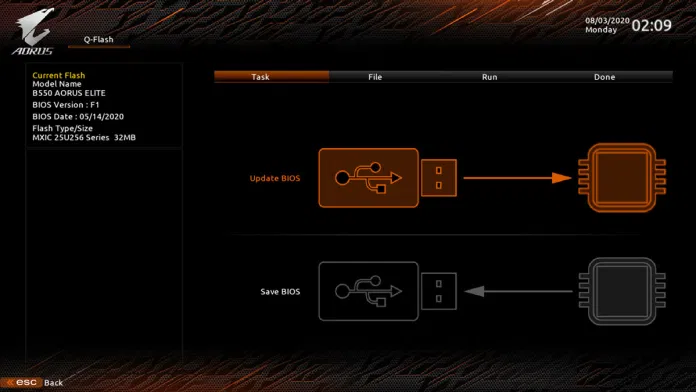
\includegraphics[scale = 0.5]{img/BIOS2.png}
            \caption{Interfaz gráfica de la BIOS}
          \end{figure}
        \newpage
          \subsubsection{Configuración del BOOT menú de la BIOS}
            Para acceder al \textbf{BOOT menú}, solo tendremos que navegar con las teclas de las flechas de nuestro teclado hasta la ventana de \textit{BOOT}, una vez ahí tendremos la opción de \textit{Boot Option Priorities}, que nos dice la prioridad de arranca 
            de nuestro PC. Nosotros pondríamos en \textbf{Boot Option \#1} la opción que queramos en que arranque por defecto.
            \begin{figure}[h]
              \centering
              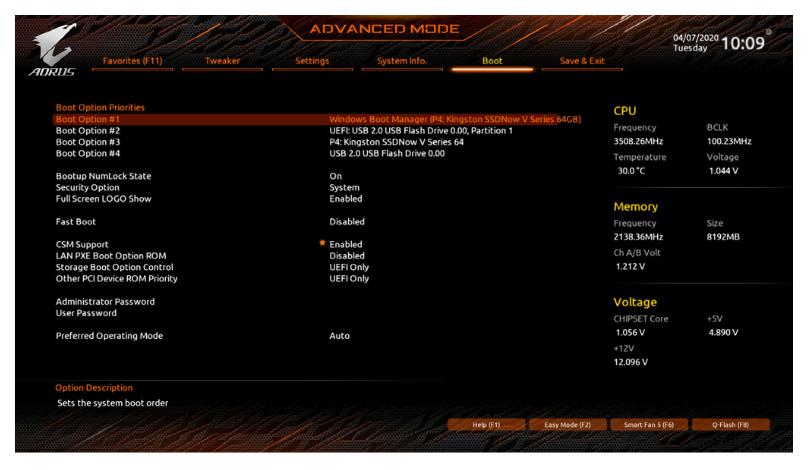
\includegraphics[scale = 0.4]{img/bootMenu.png}
              \caption{Ventana BOOT de la BIOS}
            \end{figure}
          \subsubsection{Configuración de Periféricos}
            Para acceder a la configuración donde nos encontramos nuestro periféricos, solo tendremos que ir a la ventana de \textbf{SETTINGS} y despues acceder a la sección que pone \textbf{IO ports}, una vez dentro, tendremos acceso al control de cualquier Periférico 
            que esté conectado a nuestra placa.
            \begin{figure}[h]
              \centering
              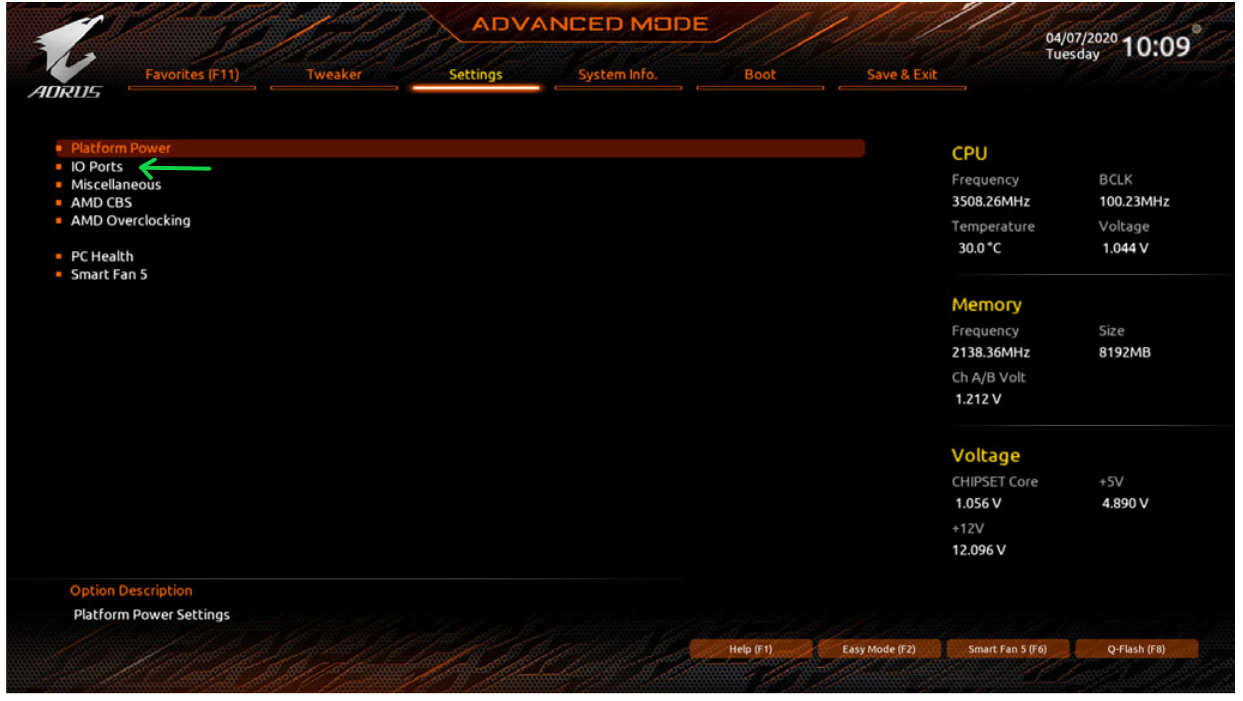
\includegraphics[scale = 0.3]{img/io_bios.png}
              \caption{Ventana de 'Settings' de la BIOS}
            \end{figure} 
      \newpage
        \subsubsection{Configurar la Virtualización}
            Para acceder a la configuración de la \textit{Virtualización}, primero accedemos a la ventana \textbf{TWEAKER} y posteriormente continuamos hasta la sección\\ \textbf{'ADVANCED CPU SETTINGS'}.\\\\
            \begin{figure}[h]
              \centering
              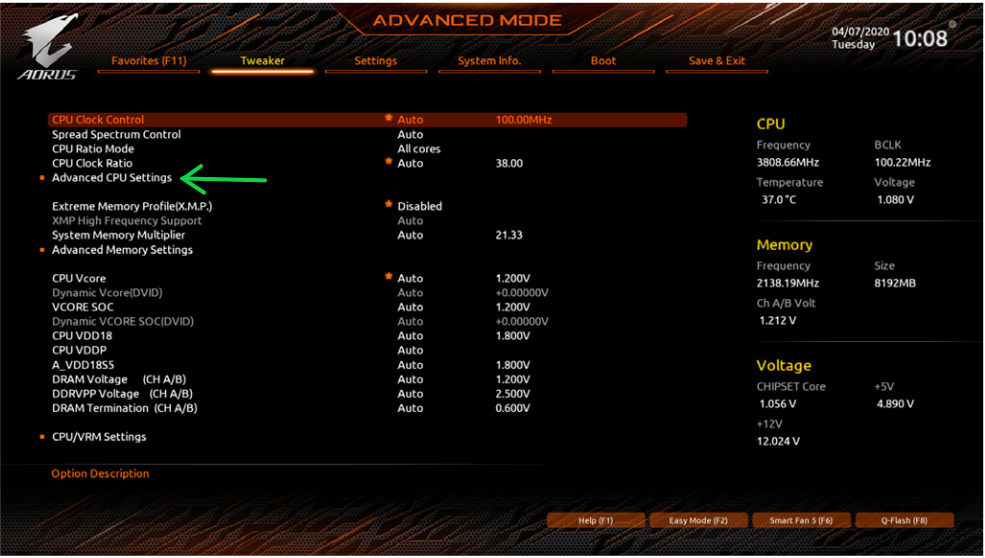
\includegraphics[scale = 0.5]{img/tweaker.png}
              \caption{Ventna 'Tweaker' de la BIOS}
            \end{figure}
            \\Una vez dentro, solo quedará buscar la función \textbf{SVM MODE}, y ponerlo en \textit{'ENABLE'}. Ya que por defecto viene con la configuración en \textit{'DISABLE'}.
\end{document}